\section{Materials and Methods}

\subsection{Hit-and-Run}
The Hit-and-Run algorithm used for sampling in a convex body $K$, was introduced by Smith in 1984 \cite{Smith}. The mixing time is known to be $\mathcal{O}^*(n^2R^2/r^2)$, where $R$ and $r$ are the radii of the inscribed and cicumscribed ball of $K$ respectively \cite{Dyer, Lovasz}.
In the case of the muscles of a limb, we are interested in the polygon $P$ that is given by the set of all possible activations $\textbf{a} \in \mathbb{R}^n$ that satisfy
\[\textbf{f} = A\textbf{a}, \textbf{a} \in [0,1]^n,\]
where $\textbf{f} \in \mathbb{R}^m$ is a fixed force vector and $A = J^{-T}RF_m \in \mathbb{R}^{m \times n}$. $P$ is bounded by the unit $n$-cube since all variables $a_i$, $i \in [n]$ are bounded by 0 and 1 from below, above respectively.

Consider the following $1 \times 3$ example.
\begin{align*}
&1 = \frac{10}{3}a_1 - \frac{53}{15}a_2 + 2a_3 \\
&a_1, a_2, a_3 \in [0,1],
\end{align*}
the set of feasible activations is given by the shaded set in Figure \ref{fig_hr}.

\begin{figure}[ht]
   \begin{center}
    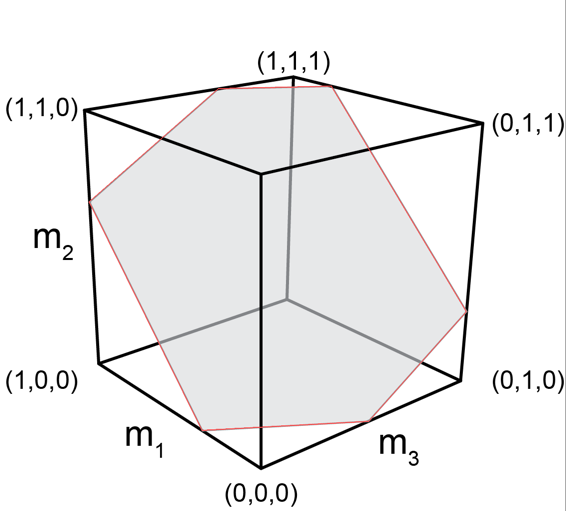
\includegraphics[width=0.25\textwidth]{feasibleactivation.png}
  \end{center}
  \caption{Feasible Activation}
  \label{fig_hr}
\end{figure}

The Hit-and-Run walk on $P$ is defined as follows (it works analogously for any convex body). 
\begin{enumerate}
\item Find a given starting point $\textbf{p}$ of $P$ (Figure \ref{fig_hr1}) .
\item Generate a random direction through $\textbf{p}$ (uniformly at random over all directions) (Figure \ref{fig_hr2}).
\item Choose the next point of the sampling algorithm uniformly at random from the segment of the line in $P$ (Figure \ref{fig_hr3}). 
\item Repeat from $(b)$ the above steps with the new point as the starting point (Figure \ref{fig_hr4}).
\end{enumerate}


\begin{figure}[ht]
   \begin{center}
    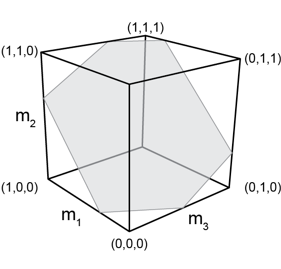
\includegraphics[width=0.25\textwidth]{HR1.png}
      \caption{Inner Point}
      \label{fig_hr1}
    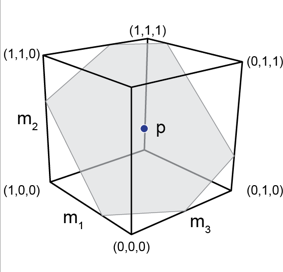
\includegraphics[width=0.25\textwidth]{HR2.png}
    \caption{Direction}
      \label{fig_hr2}
    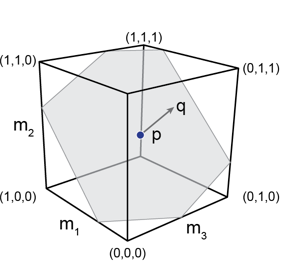
\includegraphics[width=0.25\textwidth]{HR3.png}
    \caption{Endpoints}
      \label{fig_hr3}
    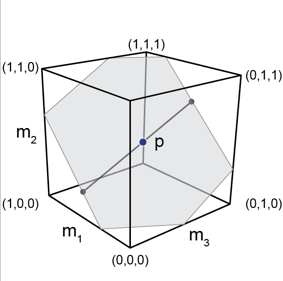
\includegraphics[width=0.25\textwidth]{HR4.png}
    \caption{New Point}
      \label{fig_hr4}
  \end{center}
\end{figure}

\begin{figure}[ht]
   \begin{center}
    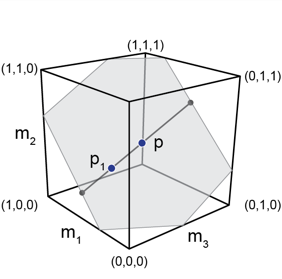
\includegraphics[width=0.25\textwidth]{HR5.png}
      \caption{Uniform Distribution}
      \label{fig_hr5}
  \end{center}
\end{figure}


The implementation of this algorithm is straight forward except for the choice of the random direction. How do we sample uniformly at random (u.a.r.) from all directions in $P$? Suppose that $\textbf{q}$ is a direction in $P$ and $p \in P$. Then by definition of $P$, $\textbf{q}$ must satisfy $\textbf{f} = A(\textbf{p}+\textbf{q})$. Since $\textbf{p} \in P$, we know that $\textbf{f} = A\textbf{p}$ and therefore 
\[\textbf{f} = A(\textbf{p} + \textbf{q}) = \textbf{f} + A\textbf{q}\]
and hence
\[A\textbf{q} = 0.\]

We therefore need to choose directions uniformly at random from all directions in the vectorspace 
\[V = \{\textbf{q} \in \mathbb{R}^n | A\textbf{q} = 0\}.\]

As shown by Marsaglia this can be done as follows \cite{Marsaglia}.

\begin{enumerate}
\item
Find an orthonormal basis $b_1, \dots, b_r \in \mathbb{R}^{n}$ of $A\textbf{q} =0$.
\item
Choose $(\lambda_1, \dots, \lambda_r) \in \mathcal{N}(0,1)^n$ (from the Gaussian distribution).
\item
$\sum_{i=1}^r \lambda_i b_i$ is a u.a.r.\ direction.
\end{enumerate}

A basis of a vectorspace $V$ is a minimal set of vectors that generate $V$, and it is orthonormal if the vectors are pairwise orthogonal (perpendicular) and have unit length. Using basic linear algebra one can find a basis for $V = \{A\textbf{q} = 0\}$ and orthogonalize it with the well known Gram-Schmidt method (for details see e.g.\ \cite{Robertson}). Note that in order to get the desired u.a.r.\ distribution the basis needs to be orthonormal. For the limb case we can safely assume that the rows of $A$ are linearly independent and hence the number of basis vectors is $n-m$.


\begin{figure}[ht]
   \begin{center}
    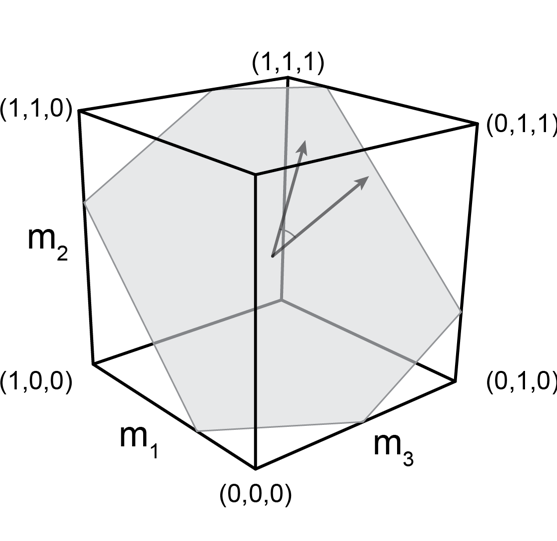
\includegraphics[width=0.25\textwidth]{somebasis.png}
      \caption{Some Basis}
      \label{fig_somebasis}
    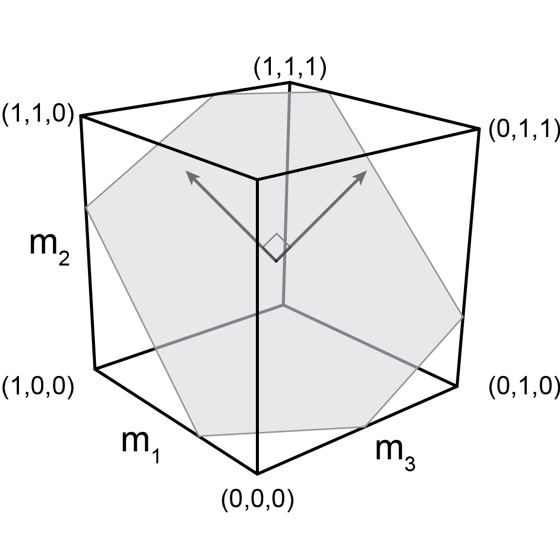
\includegraphics[width=0.25\textwidth]{orthobasis.png}
    \caption{Direction}
      \label{Orthonormal Basis}
  \end{center}
\end{figure}

\subsection{Mixing and Stopping Time}
In this section we discuss the stopping time of the Hit and Run algorithm. How many steps are necessary to reach an approximate uniform distribution? The theoretical bound $\mathcal{O}^*(n^2R^2/r^2)$ given in \cite{Lovasz} has a very large hidden coefficient which makes the algorithm almost infeasible in lower dimensions.

These bounds hold for general convex sets. For convex polygons, as in our case, Ge et al.\ showed experimentally that up to about 40 dimensions, 10 million random points suffice to get a close to uniform discussion \cite{Ge}. 
For our case we generate 10 million points and also test whether the mean of each coordinate converges and whether the upper and lower bounds for each coordinate are met. 
In detail for the mean we see that it converges after ?? steps.
For the upper and lower bounds of the activation we can solve two linear program for each coordinate of $\textbf{a}$ to find the upper and lower bounds of each $a_i$.
We see that those theoretical bounds match the experimentally obtained bounds.

\subsection{Starting Point}
To find a starting point in 
\[\textbf{f} = A\textbf{a}, \textbf{a} \in [0,1]^n,\]
we only need to find a feasible activation vector. For the hit and run algorithm to mix faster, we do not want the starting point to be in a vertex of the activation space. Therefore we solve the the following linear program.

\begin{equation}\label{eq:LP_r}
\begin{array}{lrcl}
\mbox{maximize} & \sum_{i=1}^n \epsilon_i \\ 
\mbox{subject to} & \textbf{f} &=& A\textbf{a}\\
  & a_i &\in& [\epsilon_i, 1- \epsilon_i], \hspace{5mm} \forall i \in \{1,\dots,n\}  \\
  & \epsilon_i &\geq& 0, \hspace{5mm} \forall i \in \{1,\dots,n\}.  
\end{array}
\end{equation}

This approach can still fail in theory, but this method has the choose $\epsilon_i > 0$ and therefore $a_i \neq 0$ or $1$. Since for all vertices of the feasible activation space lie on the boundary of the $n$-cube, at least $n-m$ muscles must have activation $0$ or $1$. Documentation is included in our supplementary information.